
%%%%%%%%%%%%%%%%%%%%%%% file typeinst.tex %%%%%%%%%%%%%%%%%%%%%%%%%
%
% This is the LaTeX source for the instructions to authors using
% the LaTeX document class 'llncs.cls' for contributions to
% the Lecture Notes in Computer Sciences series.
% http://www.springer.com/lncs       Springer Heidelberg 2006/05/04
%
% It may be used as a template for your own input - copy it
% to a new file with a new name and use it as the basis
% for your article.
%
% NB: the document class 'llncs' has its own and detailed documentation, see
% ftp://ftp.springer.de/data/pubftp/pub/tex/latex/llncs/latex2e/llncsdoc.pdf
%
%%%%%%%%%%%%%%%%%%%%%%%%%%%%%%%%%%%%%%%%%%%%%%%%%%%%%%%%%%%%%%%%%%%


\documentclass[runningheads,a4paper]{llncs}

\usepackage[english]{babel}
\usepackage[numbers]{natbib}
\usepackage{ifpdf}
\usepackage{amssymb}
\usepackage{graphicx}
\usepackage{subfigure}
\usepackage{epsfig}
\usepackage[toc,page]{appendix}
\usepackage{verbatim}

%\usepackage[numbers]{natbib}
\setcounter{tocdepth}{3}

\usepackage{url}

\makeatletter
\newcommand\appendix@section[1]{%
  \refstepcounter{section}%
  \orig@section*{Appendix \@Alph\c@section: #1}%
  \addcontentsline{toc}{section}{Appendix \@Alph\c@section: #1}%
}
\let\orig@section\section
\g@addto@macro\appendix{\let\section\appendix@section}
\makeatother

\urldef{\mailsa}\path|{alfred.hofmann, ursula.barth, ingrid.haas, frank.holzwarth,|
\urldef{\mailsb}\path|anna.kramer, leonie.kunz, christine.reiss, nicole.sator,|
\urldef{\mailsc}\path|erika.siebert-cole, peter.strasser, lncs}@springer.com|    
\newcommand{\keywords}[1]{\par\addvspace\baselineskip
\noindent\keywordname\enspace\ignorespaces#1}

% Audit-Bear macros
%Space saving macros
% Space saving List environment for enumerations.
\newcounter{myctr}
\newenvironment{mylist}{\begin{list}{\arabic{myctr}.}
{\usecounter{myctr}
\setlength{\topsep}{1mm}\setlength{\itemsep}{0.25mm}
\setlength{\parsep}{0.1mm}
\setlength{\itemindent}{0mm}\setlength{\partopsep}{0mm}
\setlength{\labelwidth}{15mm}
\setlength{\leftmargin}{4mm}}}{\end{list}}

% Space saving List environment for descriptions.
\newenvironment{mydesc}{\begin{description}
\setlength{\topsep}{0mm}\setlength{\itemsep}{0mm}
\setlength{\parsep}{0mm}\setlength{\parskip}{0mm}
\setlength{\partopsep}{0mm}
}{\end{description}}

% Space saving List environment for itemizing
\newenvironment{myitemize}{\begin{list}{$\bullet$}
{\setlength{\topsep}{1mm}\setlength{\itemsep}{0.25mm}
\setlength{\parsep}{0.1mm}
\setlength{\itemindent}{0mm}\setlength{\partopsep}{0mm}
\setlength{\labelwidth}{15mm}
\setlength{\leftmargin}{4mm}}}{\end{list}}

\newcommand{\smvertspace}{\vspace*{-3mm}}
\newcommand{\medvertspace}{\vspace*{-5mm}}
\newcommand{\bigvertspace}{\vspace*{-7mm}}

\newcommand{\smsubsubsection}[1]{\smvertspace\subsubsection{#1}}
\newcommand{\smsubsection}[1]{\smvertspace\subsection{#1}}
\newcommand{\smsection}[1]{\smvertspace\section{#1}}


\newcommand\cks[1]{\emph{CKS: #1}}





\begin{document}

\mainmatter  % start of an individual contribution

% first the title is needed
\title{Automated Election Auditing of DRE Audit Logs}

% a short form should be given in case it is too long for the running head
\titlerunning{Automated Analysis of Election Audit Logs}

% the name(s) of the author(s) follow(s) next
%
% NB: Chinese authors should write their first names(s) in front of
% their surnames. This ensures that the names appear correctly in
% the running heads and the author index.
%
\author{Patrick Baxter\inst{1} \and
Anne Edmundson\inst{2} \and
Keishla Ortiz\inst{3} \and
Ana Maria Quevedo\inst{4} \and\\
Samuel Rodr\'{i}guez\inst{5} \and
Cynthia Sturton\inst{6} \and
David Wagner\inst{6}}
%
\authorrunning{Automated Analysis of Election Audit Logs}
% (feature abused for this document to repeat the title also on left hand pages)

% the affiliations are given next; don't give your e-mail address
% unless you accept that it will be published
\institute{Clemson University \and 
Cornell University \and
University of Puerto Rico-Arecibo \and
Miami Dade College \and
University of Puerto Rico-Mayag\"uez \and
University of California-Berkeley}

%
% NB: a more complex sample for affiliations and the mapping to the
% corresponding authors can be found in the file "llncs.dem"
% (search for the string "\mainmatter" where a contribution starts).
% "llncs.dem" accompanies the document class "llncs.cls".
%

\toctitle{Lecture Notes in Computer Science}
\tocauthor{Authors' Instructions}
\maketitle

\smvertspace
\begin{abstract}
The voting audit logs produced by electronic voting systems contain information that is useful for uncovering procedural errors and election anomalies, but they are currently unwieldy and difficult for election officials to use in post-election audits. In this work, we develop new methods to analyze these audit logs for the detection of both procedural errors and system deficiencies. Our methods can be used to detect votes that were not included in the final tally, machines that may have experienced hardware problems during the election, and polling locations that closed late. We tested our analyses on data from the South Carolina 2010 elections and were able to uncover, solely through the analysis of audit logs, that there were 1127 votes not counted in the certified totals in Richland County, South Carolina. We created a public web application that applies these methods to uploaded audit logs and generates useful feedback on any detected issues.
\keywords{electronic voting systems, audit logs}
\end{abstract}

\section{Introduction}
Your intro goes here.

\subsection{Sub-section title}
Maybe your introduction has subsections.

\smsection{Background}
\label{sec:background}
\smvertspace
\subsection{Introduction to the iVotronic DRE}
\smvertspace
A brief description of the iVotronic's functionality and its main
system components follows. 

\begin{itemize} 
\item \textbf{Voting terminal.} The voting terminal is a stand-alone
  touchscreen voting unit.  The terminal is equipped with an internal
  battery, which keeps the unit operational in the event of a power
  failure, and a removable compact flash card, which is used to store
  audit data and ballot images (cast vote records). Typically, each
  polling location is assigned several iVotronic machines.

\item \textbf{Personalized Electronic Ballot (PEB).} The PEB is a
  proprietary cartridge designed by ES\&S to operate the iVotronic
  terminal.  When the PEB is placed in the machine, the terminal and
  the PEB can communicate through an infrared port.  Typically,
  counties deploy two types of PEBs to the precinct: a) a master PEB
  and b) an activator PEB. Both types of PEBs have the same
  functionality, however, poll workers are trained to keep them
  separate and use them for different purposes. 
    \begin{itemize}
    \item \textbf{Master PEB.}  Poll workers use the master PEB to
      open polls on election day. The same
      master PEB should be used to open all terminals in the polling
      location. In the same fashion, the master PEB should be used to
      close all terminals in the polling location at the end of the
      voting day. When a terminal is closed, it uploads its vote
      totals onto the PEB inserted into it. The PEB accumulates the precinct
      totals so that they can later be uploaded and included in the
      official tally. 
    \item \textbf{Activator PEBs.}  Activator PEBs are used by  poll
      workers to activate ballots for voters. Election officials
      provide each precinct with multiple activator PEBs.  
    \end{itemize}
\end{itemize}
Internally, all PEBs at the precinct are identical. The only
difference between them is the color of the rubber band on their
exterior. Thus, a master PEB can be used to activate a voter's ballot
and an activator PEB can be used to open and close terminals; however,
as a matter of procedure and training, they should not be used this
way. If an activator PEB is used to close terminals, the precinct vote
totals may be only partially uploaded to the aggregated totals on
election night. Poll workers are trained so that they put the master
PEB, CF cards and precinct's totals tapes in a designated bag that is
transported to Election Central after polls close.  Activator PEBs
used to close terminals may be left behind and their vote data not
added to the certified count. This has happened in the past and it causes
significant delays in the reporting of election
results~\cite{Buell2011,Mazella2002}.  

\begin{itemize}
\item \textbf{Removable Compact Flash (CF) card.} The CF cards are
  programmed at Election Central and installed in the back of the
  voting terminal prior to deployment at the polling location. They contain files
  read by the voting terminal during the voting process and store the event log
  and ballot images when the terminal is closed for voting. Once the polls 
  close, the CF cards are removed from the back of the terminal and
  delivered to election headquarters on election night.  
\end{itemize}

\subsection{iVotronic Audit Data}
\smvertspace
The ES\&S voting solution produces many log files, but in our analysis we focus
on three: the event log (EL152.lst), the ballot image file (EL155.lst), and the
system log  (EL68a.lst).    

The event log (EL152.lst) contains audit log entries from each
iVotronic terminal used in the election.  The log  records, in
chronological order, all events that occurred on that machine during the
election. It typically begins at election headquarters, before the
election, with a \textquotedblleft clear and
test\textquotedblright \hspace{1 mm} of the terminal to delete
previous election data from the terminal's memory. It also records all
election day events, including polls open and polls closing and the
number of ballots cast.  Each event log entry includes the iVotronic's
terminal serial number, the PEB's serial number, the date and time,
the event that occurred and a description of the event. %An excerpt of
%an event log is given in  Appendix~\ref{app:el}. 
 
The ballot image file (EL155.lst) contains all ballot images saved by
the iVotronic terminals during the voting process. An ES\&S ballot image
is a list of all choices made for each vote cast; it is not a scanned
or photographic image. The ballot images are segregated by precinct and
terminal where the votes were cast. The ballots are saved in a random
order to protect the privacy of the voter.  %An excerpt of a ballot image
%file is given in Appendix~\ref{app:bi}
 
The system log listing file (EL68a.lst) chronologically tracks activity
in the election reporting database at the election headquarters. Its
entries reflect the commands executed by the operators during
pre-election testing, election night reporting, post-election testing
and canvassing. It also contains the totals accumulated in the various
precincts during election night reporting, as well as any warnings or
errors reported by the software during the tabulation process.
The system log also tracks the uploading of PEBs and CF cards to the
election reporting database. Manual adjustment of precinct totals are
also recorded in the system log file. %An excerpt of a system log file is
%given in Appendix~\ref{app:sl}. 

%Analyses section
%Invoke the sub-sections through the input{filename} command.
\smsection{Analysis}
\label{sec:analysis}
\smvertspace
Our system is structured as a set of analyses. Each analysis is designed to
detect one particular kind of potential problem. In this section we present a
description of our analyses.
\smsubsection{Votes Possibly Not Counted}
\smsubsubsection{PEBs Not Uploaded}
\label{sec:pebs_not_uploaded}
The precinct procedures for poll workers dictate that a single PEB
should be used to open and close all machines at a polling
location. Failure to strictly follow this protocol can lead to problems if
election workers at county headquarters upload only one PEB, expecting all
machines to be closed with the same PEB. Recall that the PEB contains the
official cumulative tally for the precint. This has happened in the past and it 
causes significant delays in the reporting of election
results~\cite{Buell2011,Mazella2002}. 

Our
tool provides an analysis that generates a list of PEBs used to collect
votes on election day. It warns election officials of any PEB, master
or non-master, that was used to close a terminal, whose data was not
uploaded to the election reporting manager (ERM) system.  

This analysis is applicable to any voting system that has components
equivalent to a PEB and a voting terminal.  It requires an event log
that records the serial number of the PEB used to close every voting
machine and the vote events processed in the voting machine, in
chronological order. It also requires a system log file that records the
serial number of every PEB uploaded to the ERM 
system. Finally, a log providing a list of terminals used in each
precinct is also required.

Our method keeps track of the serial number of the PEB used to close each voting
machine, the polling location each voting machine was assigned
to, and the total votes cast in each machine. Then, it
reports any PEB containing vote data that has not been added to the cumulative
count.  For each such PEB, our analysis reports the serial numbers of the
terminals collected by the PEB, the number of votes processed in those terminals
and the precinct's name and number. With this information, election officials
can gather the missing PEBs and collect votes from terminals not included in the
cumulative totals.

\smsubsubsection{Machines Not Closed}
Votes could also be left out of the official tally if poll workers faill to close
all voting machines. If a machine is not closed, then a PEB has
not collected its data and its votes can not be counted; our algorithm
will  detect this situation.   

This analysis requires an event log with recorded events marking the
opening and closing of each voting machine. It also requires a log
file that allows us to identify which machines were at each polling
location. In our analysis we use the event log and the ballot image
file for this information. We created a method that checks if a
machine was closed, given it was also opened for voting.  
If there are any machines that have been opened and not
closed, they are displayed to the election official.  These
inconsistencies are only detected if the machines are closed when the
CF card is still in the machine and the complete audit data, including
the closure event, is saved to the CF card and the CF card gets uploaded to the
ERM.


\smsubsection{Incomplete Audit Data}
When a machine
appears in the event log with recorded votes cast on it during
election day, but does not appear in the ballot image file, this
indicates that some ballots are missing from the ballot image
database. Incomplete DRE ballot images will prevent accurate manual
recount procedures. The reverse situation reveals the opposite
procedural error: the event log is not complete.  We developed a
technique that identifies incomplete databases.   

This analysis requires an event log and a ballot image file, where
both files record machine serial numbers for any events and ballots
cast.  Our analysis crosschecks these files for inconsistencies by comparing the
number of ballots in the ballot image file with the number of cast vote events
in the event log. If the numbers do not match we report file 
inconsistencies and provide the user with the machine serial number
and the conflicting vote counts.      

\smsubsection{Polling Location Related Analysis}
%\subsubsection{Polling Locations that Closed Late}
In the United Stated, poll closing hours vary from 6pm to 9pm depending on the
state~\cite{Info2007}. Some state statutes allow the voters waiting in
line at poll closing time to cast their ballots at the precinct, requiring those
polling locations to stsay open late. If election officials knew which polling
places were likely to 
experience long lines they could deploy more equipment or personnel to
those locations. This analysis can assist them by providing
information about long lines that occurred in the current election, which they
could use to make predictions about where
long lines might occur in future elections.

This analysis gathers the time each machine was closed from the event log and
the precinct the machine was assigned to from the ballot image file
and generates a countywide chart detailing the number of polling
locations that stayed open after poll closing time and for how long. To handle
inaccurate machine date/time settings, our tool uses a time verification
algorithm described in Section 3.6 to exclude from our database any voting
machines whose time stamp is probably incorrect. 


\subsection{Hardware Issues}
\smvertspace
Next we describe ways to identify machines that have hardware problems, such as
screen calibration issues, machines with power supply problems, machines that
closed early, and machines that recorded unknown, but possibly severe events.
Analyses such as these can help officials identify machines that may require
maintenance or need to be replaced.  

\smsubsubsection{Calibration Errors}
The first of these analyses detects machines with recurring calibration errors
and machines that recorded votes while possibly not calibrated.  When
a machine is not calibrated, it may not
correctly capture the voter's intent; if the calibration is inaccurate, a voter
may think they are voting for candidate X, but the machine may record a vote for
candidate Y.  The importance lies not only in the fact that voters' intents may
not be recorded, but also in the possibility that this error may not issue a
warning to the voter when it happens.   

To allow this analysis, the event log needs to record a collection of
events. These events include: a machine's screen is not calibrated or
the screen cannot be read, a screen is calibrated by a technician, and
a vote is cast.  In addition, it is not sufficient to have
chronologically ordered events in the log; it is essential that the
events in the event log have accurate date and time stamps so that we can
restrict our analysis to calibration issues
that occur on election day.  To find the polling location of the
machines used, the ballot images file should also be supplied.  

We detect the calibration errors by searching the event log for votes cast after
a machine 
recorded a bad calibration event (e.g., ``Warning - cannot read terminal
screen'')  and before the screen has been recalibrated. If a vote cast event
occurs before any recalibration event,
then the machine is reported to the election official, as this means
there was at least one vote cast when the machine's screen may not
have been calibrated.  

\smsubsubsection{Power Supply Errors}
The second analysis regarding hardware problems looks for machines with possible
power supply issues.  We report machines that experience a higher-than-average
number of events related to the Internal Power Supply. One possibility is that
these machines have a low battery supply, which could lead to an automatic
shutdown.  If a machine shuts down because it no longer has enough power to
continue working, the polling location will have fewer machines.  In the case
where a polling location has limited resources, it is more likely that there
will be long lines of voters waiting to vote; some may leave without voting.   

In order to run this analysis, the event log must contain events related to
power supply or low battery power; having a correct date and time stamp is also
a necessity.  The ballot image file provides the locations of each machine used,
which is essential in this analysis. Currently, the publicly available iVotronic
manuals do not describe the meaning of the events that appear in the event log.
Because of this, we had to make some educated guesses about the meaning of each
event.  We interpreted the event, \textquotedblleft Terminal shutdown - IPS
Exit\textquotedblright \hspace{1 mm} as a power supply-related event because IPS
stands for Internal Power Supply~\cite{email2010}.  This analysis keeps track of
every machine in the event log and how many instances of the previously stated
event occur on each machine.  Having a higher-than-average number of this event
type should cause concern because it indicates there was an ongoing problem that
was not solved. A machine with an average number of this event is ignored
because it may be warning about a machine with a low battery, which was then
connected to a power outlet and therefore, stopped recording this event. 
Without any prior knowledge of what the \textquotedblleft
normal\textquotedblright \hspace{1 mm} number of events might be, we start by
assuming the number of events seen by any machine will follow a normal
distribution. This is a reasonable assumption because machines that are not
connected to a power supply will likely run low on battery at some point during
the approximately 12 hour day. A few machines may be connected to a power outlet
(causing unusually small numbers of this event) and a few machines may
experience low battery power to the point of automatic shutdown (causing
unusually large numbers of this event).  Assuming a normal distribution, our
analysis calculates the mean and standard deviation of the number of times this
event occurs per machine.  If a machine has an unusually large number of
instances of this event (over three standard deviations above the mean), we
consider it to have power supply issues.

\smsubsubsection{Machines that Closed Early}
We have also developed a way to detect machines that have closed early. A
machine will not shut down before poll closing time unless it is explicitly
closed by a technician or a properly trained poll worker. If a machine is closed
in this manner during election day, there may be something wrong with it
preventing its normal operation.
                  
Event logs that record dates and times accurately, as well as events
that mark a machine being closed for voting, are necessary for this
analysis. Also, it is essential to know the official time when polls
open and close. To help officials take corrective action, we need the
ballot image file to determine the location of the possibly
problematic machines. The event we search for indicates that a machine
was closed early; in the case of the iVotronic it is called:
\textquotedblleft Warning -- Terminal Closed
Early.\textquotedblright \hspace{2 mm} If an occurrence is found between
official poll opening and official poll closing times, the analysis reports the
machine that recorded it to indicate a machine that closed early.  

\smsubsubsection{Anomalous Warnings}
There may be events in the event log that would raise a red flag for election officials. This analysis will report machines that have recorded at least one of these events. The machines that experience these events should be inspected for possible hardware issues; the warning events may indicate an equipment failure or other problem that should be corrected.

Given a set of warning events, this analysis can run on any event logs that record the events in the given set. It would be beneficial to have accurate date and time stamps to narrow the analysis specifically to election day. Additionally, the ballot image file would provide information regarding which machines were used at each polling location.  In the case of the iVotronic, we flagged the following events as warning events: \textquotedblleft Warning -- PEB I/O Flag Set,\textquotedblright \hspace{1 mm} \textquotedblleft Warning -- I/O Flagged PEB will be used,\textquotedblright \hspace{1 mm} and \textquotedblleft Warning -- no valid term audit data.\textquotedblright \hspace{2 mm} Our reasoning was determined by the keyword \textquotedblleft Warning\textquotedblright \hspace{1 mm} as well as by manually analyzing the context in which these events occur in the audit logs. Due to a lack of event descriptions, there may be a set of events that appear to be warnings, but may not require any action. In any case, our analysis searches the event log for the instances of any of the above events that occur on election day and reports the machines that recorded these instances. 

\subsection{Procedural Errors}
\smvertspace
It may be beneficial to election officials if they could detect at which
locations poll workers are following the required procedures. Procedural errors
can cause many problems including lost votes, incorrect vote counts, disgruntled
voters, and long lines. A few errors that might occur are: precincts that do not
print zero tapes on the morning of election day; using a master PEB to activate
ballots; and opening and closing machines with different PEBs. If election
officials are aware of the procedures that are not being followed, they could
improve their precinct checklist. This will allow for more efficient audits as
well as a better voting experience for voters. 

\smsubsubsection{Printing Zero Tapes}
This analysis pertains to jurisdictions that require poll workers to
print at least one zero tape per polling location. The printing of a zero tape
is important to verify that the voting machines are set to zero; it
ensures that additional votes will not be included in the certified
count. In this analysis we check if this procedure is followed.

In order to run this analysis, we require both a ballot image file, which
contains the machines and precincts, and an event log.  Given an event log that
has correct date and time stamps, and an event that represents the printing of a
zero tape, we can detect if this procedure was followed.  We limit our search of
the event log to events that occurred on election day.  We have noticed that the
zero tape may be printed before or after the official poll opening time, so we
do not specify time limitations.  Our analysis groups the machines found in the
event log by polling location using the ballot images file and requires at least
one machine per polling location have this event. If none of the
machines in a polling location record this event, we report the polling location
and the corresponding machines. 
%\cks{If multiple PEBs are used to open machines, but only one is used
%  for the zero tape, do you catch it?}

\smsubsubsection{Ballot Activation with a Master PEB}
Another procedure that should be avoided is using a master PEB to activate ballots for voters.  Poll workers should be using non-master (activator) PEBs to activate ballots for the reasons outlined in Section \ref{sec:background}.

This analysis focuses on procedures related to the use of the PEB and the voting
machine; it is applicable to other voting systems that use a similar process.
To detect violations of this procedure, the analysis requires that the event log
records votes being cast, machines being opened and closed, as well as the PEB
number used for each event.  Through this analysis we assign each machine a
master PEB: the PEB used to open and close the machine. Then, we check to see if
any votes were activated on each 
machine using the master PEB.  If we find any such cases, we report them.  In
the case that two different PEBs were
used to open and close the machine, our algorithm
checks both and if a ballot was activated with either one,
then that machine and PEB are reported.  


\smsubsubsection{Opening and Closing a Machine with Different PEBs}
\label{sec:opening_closing_diff_pebs}
Along the same lines, we report incidents of opening and closing a
machine with different PEBs. A machine should be opened and closed
with the master PEB; if not, it may be more likely that the non-master
PEB used for closing machines and its corresponding votes will be left behind at the precinct.  Poll workers are trained so that they put the master PEB, CF cards, and printed precinct tape in a designated bag, which is transported to election central after the precinct is closed.  

The requirements for this analysis are similar to the analysis discussed above.
As this analysis works with procedural errors concerning the interaction between
PEBs and the machine, it applies to systems that work in the same manner.  The
event log should contain events signaling the opening and closing of each
machine and the PEB used for each event.  In this analysis, we find the serial
numbers of the PEBs used to open and close each machine.  If the two PEBs have
conflicting numbers, then we report the machine and PEB serial numbers.  If the
PEBs are the same, then the correct procedure was followed and no machines are
reported.  


\smsubsubsection{Anomalous Vote Cancelled Events}
There may be
many reasons why votes are cancelled. According to the iVotronic’s event logs
there are seven options for canceling a ballot. Depending on the reason chosen, it
might be possible to identify procedural errors.  For example, if there are any
instances of canceling a ballot due to a printer problem, it could be an
indicator of a procedural error because ballots are not normally printed. In other
cases, if there is a large number of a specific reason, such as having the wrong
ballot, this could indicate the poll workers are repeatedly issuing the wrong
ballot or the terminal is experiencing calibration issues.  

This analysis has a higher potential to be used on other voting systems than the
previous two analyses.  It only requires that the event log record
votes being cancelled, and reasons as to why the vote is being cancelled.  This
analysis would perform best if the date and time stamp were accurate as well.
For each machine, we associate with it the number of each type of vote
cancellation recorded and report the
machines that had at least one vote cancellation event type that occurred an
unusually high number of times. In our analysis, an \textquotedblleft unusually
high number of times\textquotedblright \hspace{1 mm} is defined as having a
number of instances greater than three standard deviations above the average for
that event type.
If it is the case, we will also report if a machine has an unusually high
number of instances for more than one vote cancellation event type, and which
event types they are.  



\smsubsection{Systematic Date and Time Errors}\label{an:date} 
\smvertspace
Correct time-stamps in the audit logs
are critical in post election audits as any incorrect time-stamps
could preclude further log analysis. 
We classify time-stamp errors into two categories: errors
resulting from incorrectly set clocks and errors resulting from apparent bugs in
the time-stamp mechanism itself. Our tool will analyze log files to
find and report errors of each category type.

This analyses requires that each event in the audit log
is marked with a time-stamp based on the machine's internal clock. If
the clock can be manually set, we require that any adjustment made to
the clock is recorded as an event in the
audit log. Additionally, opening and closing events recorded in the logs proved
useful to the analysis. It allowed the analysis to report only those
errors that occur on election day and to avoid reporting as error
any inconsistent time-stamps that occur prior to election day and are
likely the result of pre-election testing or configuration of the
machines. We developed some checks to report if any of
the above requirements are not met by the log data.

Often, an analysis of the time-stamps can produce ambiguous
results. For example, if a machine has its clock set an hour back it
is difficult to determine, from the log files alone, whether the machine
was opened early or its clock was incorrectly set. In our analysis, we
favor accurate identification of date errors over complete
identification. We want to avoid flooding the user with false or
ambiguous error reports. For this reason, we developed techniques to
remove as many ambiguities as possible and report only those
instances which we can positively identify as errors.

We perform these analyses by sequentially parsing each event in the
audit log while looking for events marking a manual clock adjustment
or an erroneous shift between two consecutive time stamps. We explain
our technique further in the following subsections.

\smsubsubsection{Incorrectly Set Dates}
This report identifies any machine that opened for election day voting
with an incorrectly set clock.  This means the opening event and
possibly all subsequent vote events were recorded with incorrect
time-stamps. This error can prevent other analyses
from properly detecting how long the polls stayed open, whether they opened on
time, or if they experienced long lines. Additionally, it may be useful for an
election official to identify counties or precincts where these errors were
particularly common so that pre-election testing procedures can be improved.
We used two different detection algorithms to identify these errors.

The first found machines that opened for voting with wildly incorrect
dates and times. In this algorithm we looked for any machine which
opened for election day voting on any date after the official election
day or any date more than one month prior to election day. This one
month threshold allowed us to avoid reporting those machines which
were legitimately opened, possibly for early voting, on a date before
the official election day. \cks{Patrick, is this the right reason for
  the one month window? Correct it if I'm wrong.}

The first algorithm found those machines whose date and time were
off by a large amount, but it will not find machines that have a
time-stamp that is off by only a small amount, perhaps just an
hour. To find those machines we used a different technique. Instead of
looking at the time of opening or closing, we instead looked for
machines whose time-stamp was manually adjusted at some point while
the machine was opened for voting. If we saw an event indicating the
time-stamp was set forward one hour, for example, we could surmise that
up until that point, the machine's clock had been one hour slow and we
could retroactively adjust the time-stamps of the earlier events for
use by our other analyses.

If a machine opens with a clock that is wrong, but by an amount
smaller than our allowed window of error (one month for slow clocks,
24 hours for fast clocks), and whose clock is not adjusted at any
point during election day, our analyses will fail to catch the
error. We decided on this window size after some trial and error with
the South Carolina data set we were working with; this size seemed to
yield the fewest false positives while still returning useful
results. Possibly, other data sets will require a different
window. This analysis could reasonably be parametrized to
allow the user to specify the desired window size if the default does
not provide useful results.

\smsubsubsection{Datetime Errors}
This report identifies anomalies in the time stamps that are not a result
of human error. In the course of our analysis of the South Carolina
data set, we found many dates that changed, seemingly at random and without
a manual date adjustment event. Sometimes these jumps were temporary
and the clock would jump back to its original time, other jumps
appeared to be permanent. These occurrences suggest an issue with the
machine itself rather than a procedural error. The cause of these errors remains
unknown, but it is concerning that these values can change arbitrarily
as they have the potential to invalidate other audit analyses.  Reporting these
anomalies may assist officials in determining which machines require
inspection by the DRE vendor.

Since events are appended in chronological order, any time-stamp that decreases
chronologically without a corresponding event indicating a manual
adjustment took place is an error and is detected by this
analysis. Forward jumps in time are not necessarily the result of an 
inconsistent time record; a machine can be shut down in a hibernation state for
weeks between events. However, given the relatively short duration of elections, jumps
forward in time, that are past a certain threshold, can reasonably be considered
erroneous. The algorithm looked for deltas between time-stamps that jump
forward by more then 33 days. With the South Carolina data set we
analyzed, this threshold seemed to
avoid including machines that were simply in hibernation between the
factory setup and election day voting. Additionally, some machines were found to have their clock set to
a type of null state where the clock stopped incrementing and marked blank
dates; therefore, our analysis looks for these errors as well.

For each error detected, the number of events associated with the error
is reported, as well as the anomalous date and the machine serial
number. The number of events associated with an error is the number
of events in the event log between the point where the anomalous clock
change occurs and the point where the clock corrects itself, if it ever
does. If the clock never corrects itself, all subsequent events in the
log are counted as associated with the error. If the clock
does correct itself, that is detected as follows. The \emph{start
event} of the anomaly is the event just prior to the event with the
anomalous time stamp.
A backward jump is presumed over if an event
appears that is chronologically forward in time compared to the start event.
A forward jump is assumed over if an event appears on the same day of the
starting event.  The zero clock anomaly is detected as returning to normal as
soon as a non-zero date appears.


\subsection{Future Analysis}
Election officials assign voting machines and supplies to each polling
location based on the number of voters registered in the precinct.
However, voter turnout can vary and as a result, some polling
locations may end up overstocked with equipment, supplies or poll
workers while others may lack resources on election day. As a result,
voters may have to wait in line before casting their vote. This is
common during mid-term and general elections~\cite{Kreitman2010,
  Slade2008, U2010}, as well as any elections with high-voter turnout.
In those circumstances, election officials might like information
about which locations experienced long lines and at what time of the
day. However, monitoring all the polling places in a large county can
be a daunting task. Therefore, providing an analysis that can analyze
DRE audit data to identify peak times at the precincts would be useful; such
information could assist election officials with the planning of
resource allocation for future elections.

\begin{comment}
This analysis reports busy locations by detecting heavily used voting terminals. It requires an event log that captures every vote cast event along with an accurate time stamp and precinct location information. In our analysis we find this information in the event log and the ballot image file. When there are consecutive ballots cast in all machines in a polling location with no time delay in between, we are able to infer that there is a steady flow of voters and possibly a line of voters waiting to use the voting machines. 
\end{comment}

However, the analysis is not quite so straightforward. The event logs
we used captured the \textquotedblleft cast vote'' event, but that
only tells us when the voter finished making their selection. In order
to know if there is any idle time between voters, we would also need
an event that notes when a new ballot is loaded into a machine. The
idle time would be the time between one \textquotedblleft cast vote''
event and the next \textquotedblleft ballot loaded''
event. Unfortunately our logs have no such \textquotedblleft ballot
loaded'' event. We are exploring the possibility of inferring the idle time by
comparing the time between cast vote events in any given time period to the time
between cast vote events at times when we can reasonably assume voters were
waiting in line and the idle time was likely close to zero.
\begin{comment}
Instead, we had to infer the idle time. We did this by
focusing on the polling locations which stayed opened after poll
closing time as we could conclude they were busy processing the voters
standing in line at that time and the time between cast vote events
includes no idle time. For those locations, we measure the time it
took voters to cast ballots during the extended poll hours. We also
calculate and keep track of the time per ballot cast during regular
poll hours. Using the Kolmogorov- Smirnov statistical test we can
determine whether the distribution of time between vote cast events
during regular poll hours, in one-hour time windows, matches the
distribution of time between vote cast events during the extended poll
hours. If the distribution of the two samples is consistent, we can
infer the possibility of long lines during the particular one-hour
time period. \footnote{The KS test starts with the null hypothesis
  that the two samples come from the same distribution, which is the
  situation we are interested in identifying. Therefore, the most we
  can say in the case that the null hypothesis cannot be rejected is, we
  cannot reject the possibility that there were long lines between a
  particular time window.} 
\end{comment}



%Implementation section
\section{Implementation}
This section describes the AuditBear tool.  Gives an overview of the workflow from the perspective of a user.  Possibly add a diagram.

%Results section
\input{results2.tex}
% Future Voting System Suggestions
\section{Future Voting System Suggestions}
[To complete by Wednesday].

% Related Work section
\section{Related Work}
Many election technology systems provide a means of auditing elections. For example, in optical scanning systems the cast ballots form a paper record of the votes cast.  On the other hand, paperless DRE machines do not provide this type of paper trail. Some DRE systems provide a Voter Verified Paper Audit Trail (VVPAT), which stores a hard copy version of each ballot cast.  A third type of audit trail, which is produced by all DREs, are the event logs stored electronically on each DRE.  In this section we discuss related work on the analysis of audit logs for post-election auditing. 

Two recent studies used event logs from the iVotronic voting system to audit elections~\cite{Buell2011,Sandler2007}. The authors of the first study~\cite{Buell2011} performed an audit of the same South Carolina elections that we analyzed. Using these audit logs, they discovered votes not included in the certified counts and problems with the audit data. They crosschecked the event log, the ballot image file, and the system log to identify unsupported votes and missing audit data.  By consulting additional audit materials, such as the printed results tapes, the authors were able to offer possible reasons and explanations as to why the problems occurred. Our work takes a slightly different approach.  We focus on developing a variety of methods to analyze the data; in addition, we automate these analyses for use by election officials.  While our tool did discover and report similar problems, we simply report what was wrong, but can not provide a possible explanation for the cause of the error as we didn't have access to printed results tapes. 

The authors of the second study~\cite{Sandler2007} provided an analysis of vote tallies using the protected count of votes on each machine and comparing this to the printed results tapes. Their report also finds date/time stamps that were most likely inaccurate.  With further investigation, they concluded that the machine hardware clock was incorrect. Our research provides analyses to identify similar problems, but in a way that could be automated. 

There has also been research on using the audit logs to analyze election-day procedure and activity. For example, one recent publication showed how event logs could be used to determine if a machine acted \textquotedblleft normally\textquotedblright on election day~\cite{Antonyan2009}. The authors of this research studied the event logs of the AccuVote Optical Scanning system and used those logs to build a finite state machine that models the sequences of events that a well-behaved machine might produce. This type of analysis would be useful to provide for the iVotronic systems that we studied. However, the AccuVote machines have considerably fewer possible event types than the iVotronics so the analysis would become considerably more complex. 

A common problem on election day, which we try to identify in our analysis, is the occurrence of long lines. Many studies have researched ways to mitigate long lines at polling locations ~\cite{Allen2006,Dow2007,Spencer2010,Wilson2008,Edel2010}.  One such study has simulated the flow of voters through the voting process~\cite{Edel2010}. The authors use this simulation to determine the optimal number of voters per voting machine, and correspondingly, the appropriate number of voting machines per polling location based on the number of registered voters at that particular location. Their work is predictive: the authors make some assumptions, such as the average time it takes to vote and when peak voting hours will occur, and use those as a basis for predicting where long lines are likely to occur. Our analysis is descriptive: given the audit logs from election day, we infer the average time it took to vote and use that information to determine whether a particular polling location experienced long lines or not. The two methods are complementary. Predictive models can be used to prevent long lines, while descriptive models can be used to check and refine the prediction algorithms. 

Voter Verified Paper Audit Trails (VVPATs) are a different type of audit log. Unlike the audit logs we used in our analyses, VVPATs are viewed and verified by the voter and are more suited to audits concerning a DRE incorrectly capturing a voter\textquoteright s intent. Our work is more concerned with identifying cases of cast votes not being included in the final count, or issues at the polling place that might prevent the voter from casting their vote in the first place. With VVPATs, as long as a certain percentage of voters do check their paper ballot~\cite{Hall2006}, the voting machine need not be assumed correct, whereas our analyses do make this assumption.

%Conclusion
\section{Conclusion}
In this study we developed a tool to analyze audit data from DRE voting machines. Our web based application, accessible to anyone, performs a variety of analyses on the audit data to detect procedural errors and system deficiencies. We replicated a previous study conducted using iVotronic audit logs collected in South Carolina after the 2010 Primary and General elections~\cite{Buell2011}. The aforementioned paper identified media devices containing votes that were not included in the certified totals. In addition, our tool can identify terminals that were not closed and their votes not uploaded to the cumulative count. This information can be very useful during the canvass process as election officials can locate the missing terminals, close them and add their votes to the election totals. 

Having performed analyses with the iVotronic logs from South Carolina, we also report statistics on polling location procedures. These statistics include: polling locations that closed late or may have experienced long lines of voters, precincts which did not report the zero tape and polling locations which used the wrong device to activate ballots on election day. Our tool can also report statistics concerning possible DRE hardware problems such as calibration issues, low battery and incorrect date and time settings. With this information election officials can improve their poll worker training or schedule voting machine repairs as needed.

%This point is going to need more work.  I'm thinking if we expand on it we might want something about Wagner's work in either our introduction or related works section.
Dr. Wagner's commissioned report ,  "Voting Systems Audit Log Study" extensively documents and evaluates many different types of audit logs produced by six different voting systems.  In the findings there were no machines that provided tools, support, or generated summary reports for analyzing audit logs.~\cite{Wagner2010}. While, the authors are very familiar with the strengths and weaknesses of the iVotronic's audit logs we would direct anyone interested in the future design of audit logs to this report.  Fully documenting the strengths and weaknesses of the iVotronic audit systems is outside the scope of this project. Our website is only the first step in creating a process for automated election auditing.  We hope that future third-party audit log  tools can build on some of this previous work to create a useful and robust solution for deriving meaningful audits directly from the logs.

We recommend that election administrators conduct routine reviews of the audit logs generated by the voting machines as they are ground truth for election disputes. By automating our analyses and making it as simple as uploading the iVotronic audit logs to a website, we believe our tool can standardize the post-election audits performed by the iVotronic system users. Our website can quickly provide intelligent feedback to election officials during the canvassing process and serve to influence future audit procedures. 

%Acknowledgements section
\section{Acknowledgments}
We thank David Wagner and Cynthia Sturton for their support and contribution.  Special thanks to Dr. Kristen Gates, National Science Foundation and the TRUST program staff.


\bibliographystyle{splncs03}
\bibliography{paper2}


\appendix
\section{Event Log File}\label{app:el} 
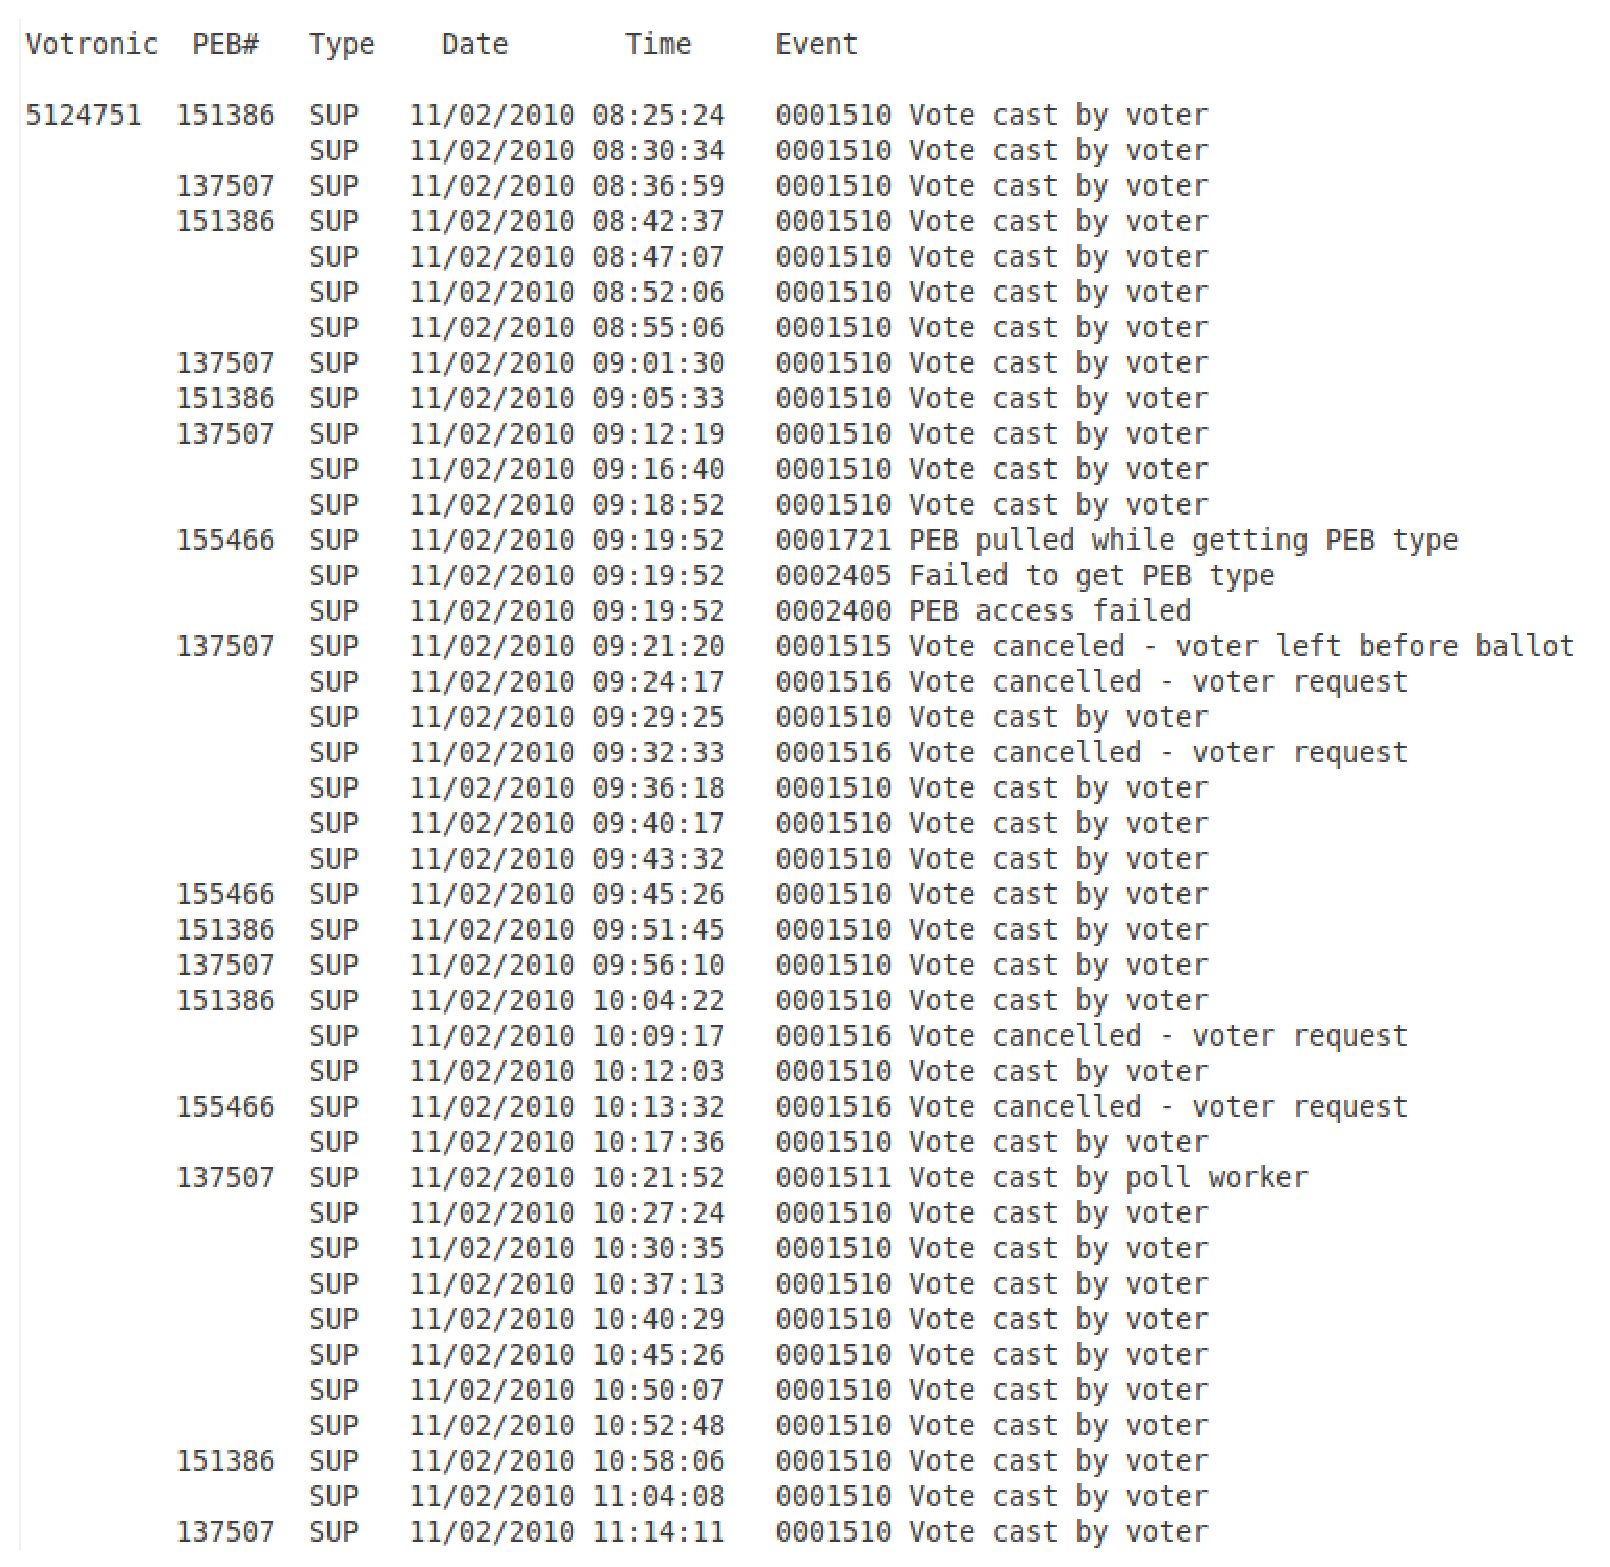
\includegraphics[width=0.7\textwidth]{eventLog}
\section{Ballot Image File}\label{app:bi}
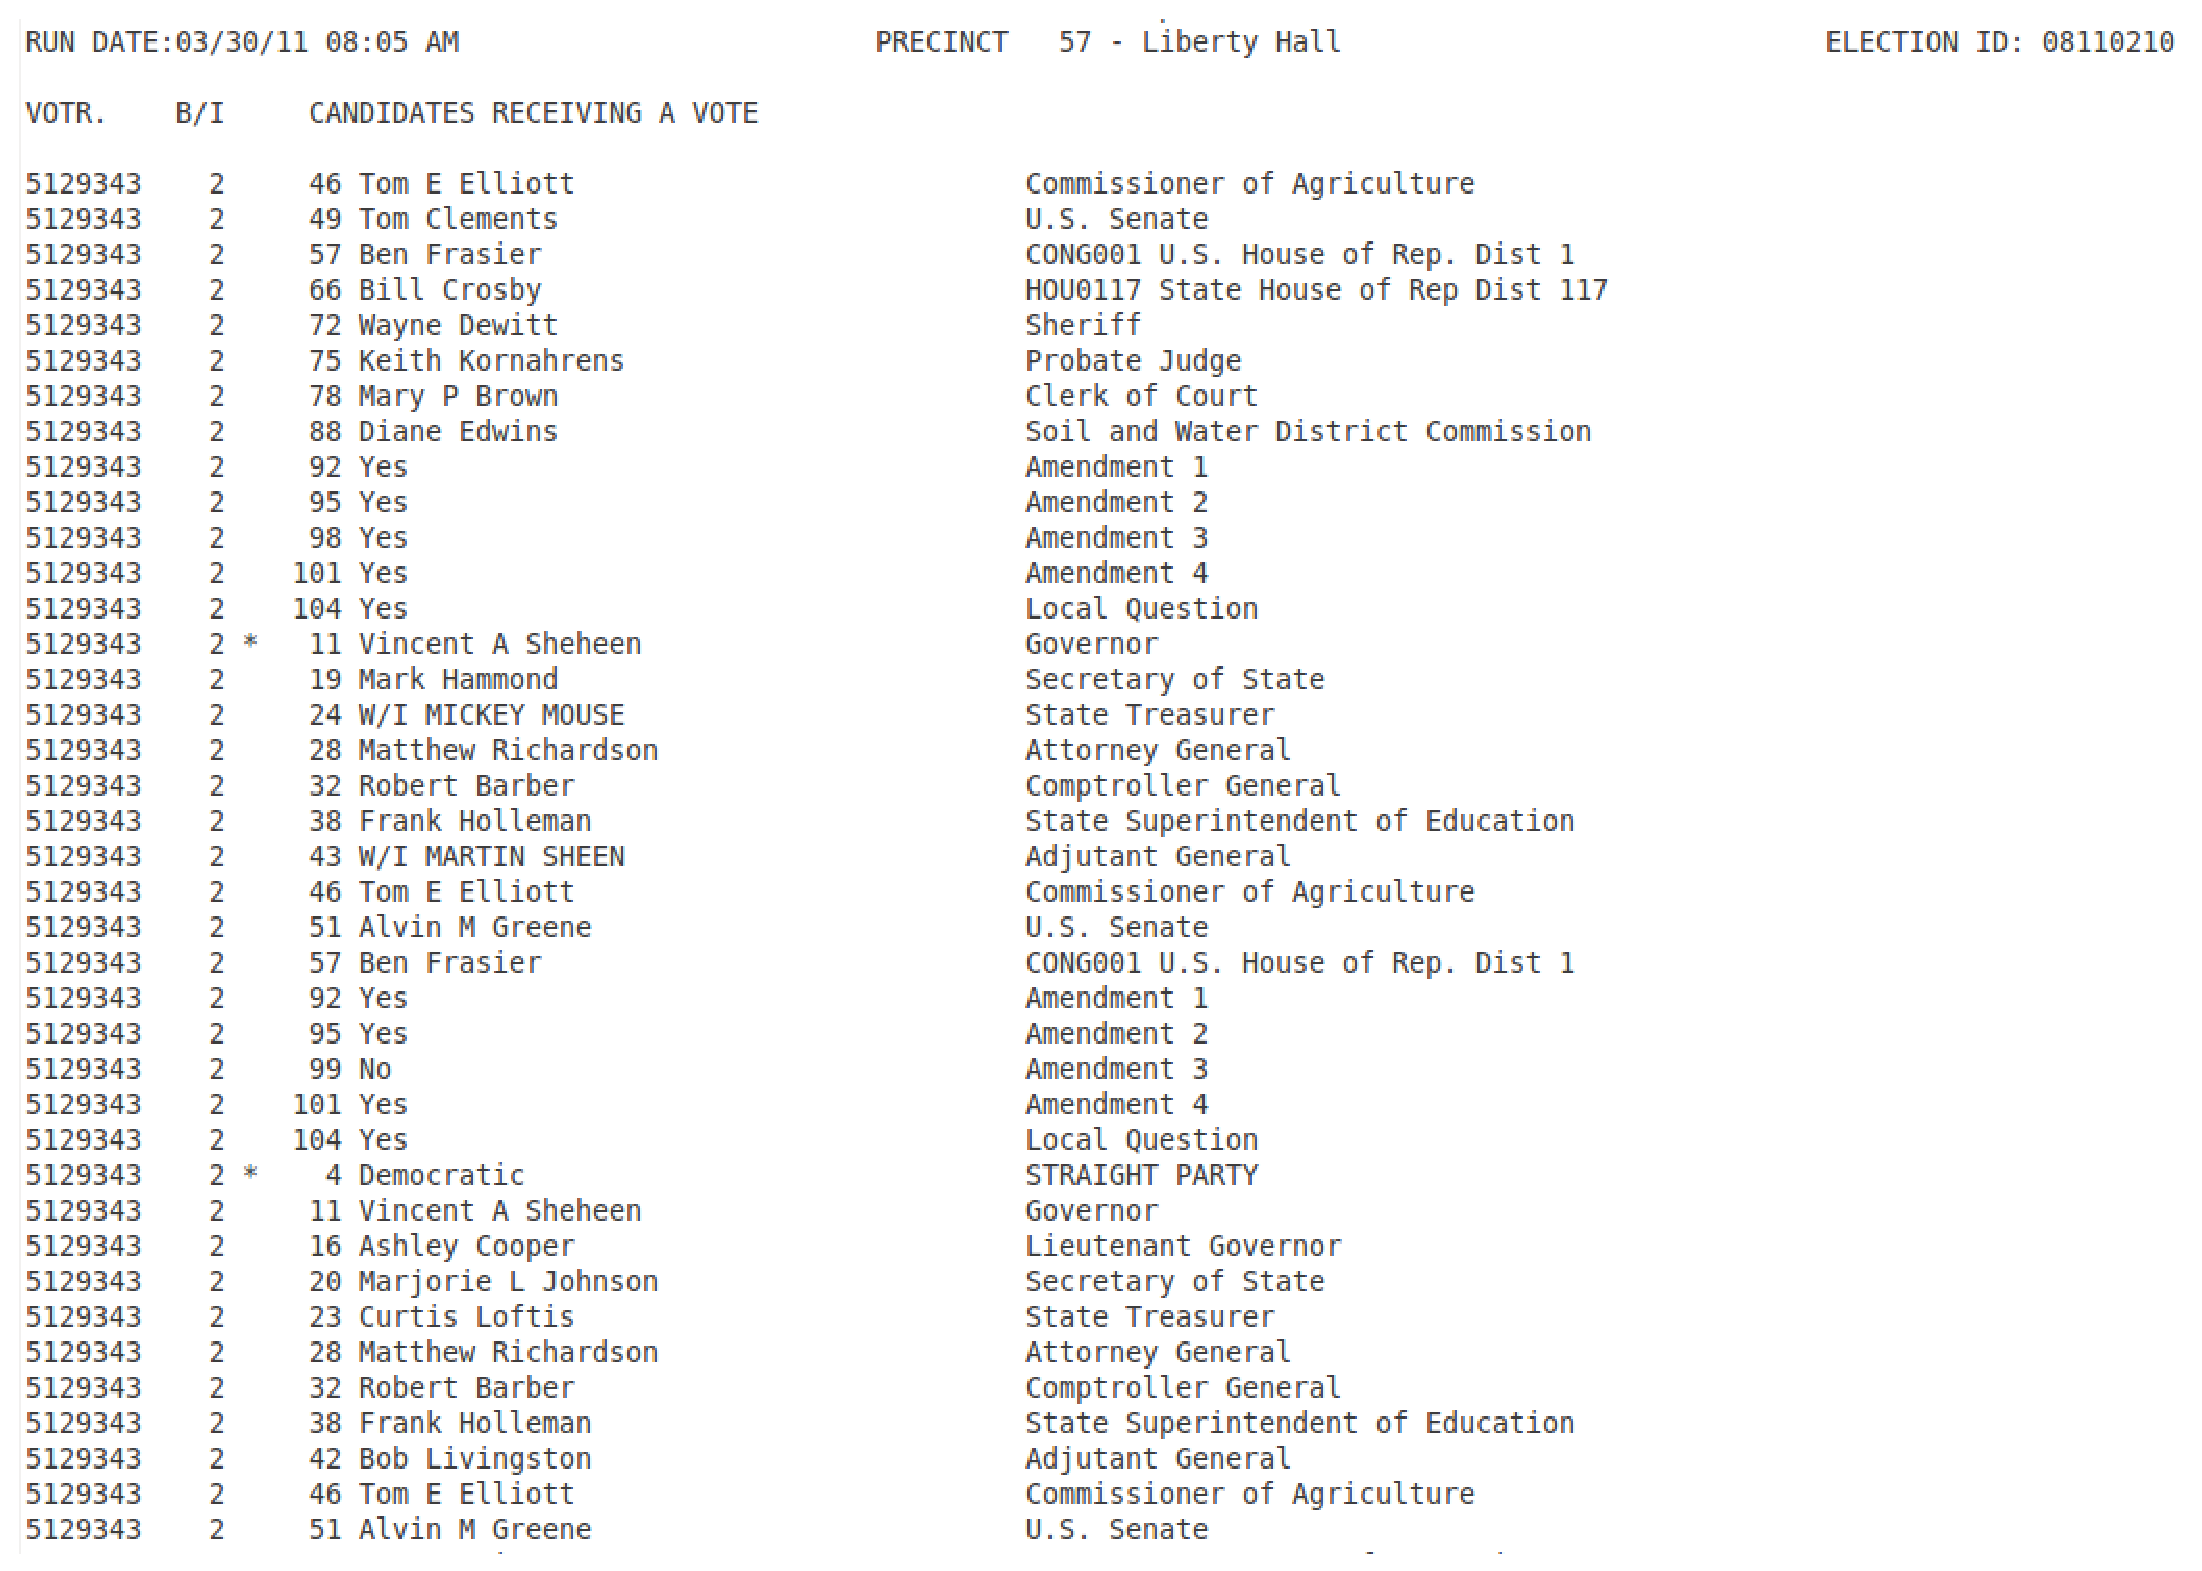
\includegraphics[width=0.7\textwidth]{ballot}
%This is app~\ref{app:bi}
\section{System Log File}\label{app:sl}
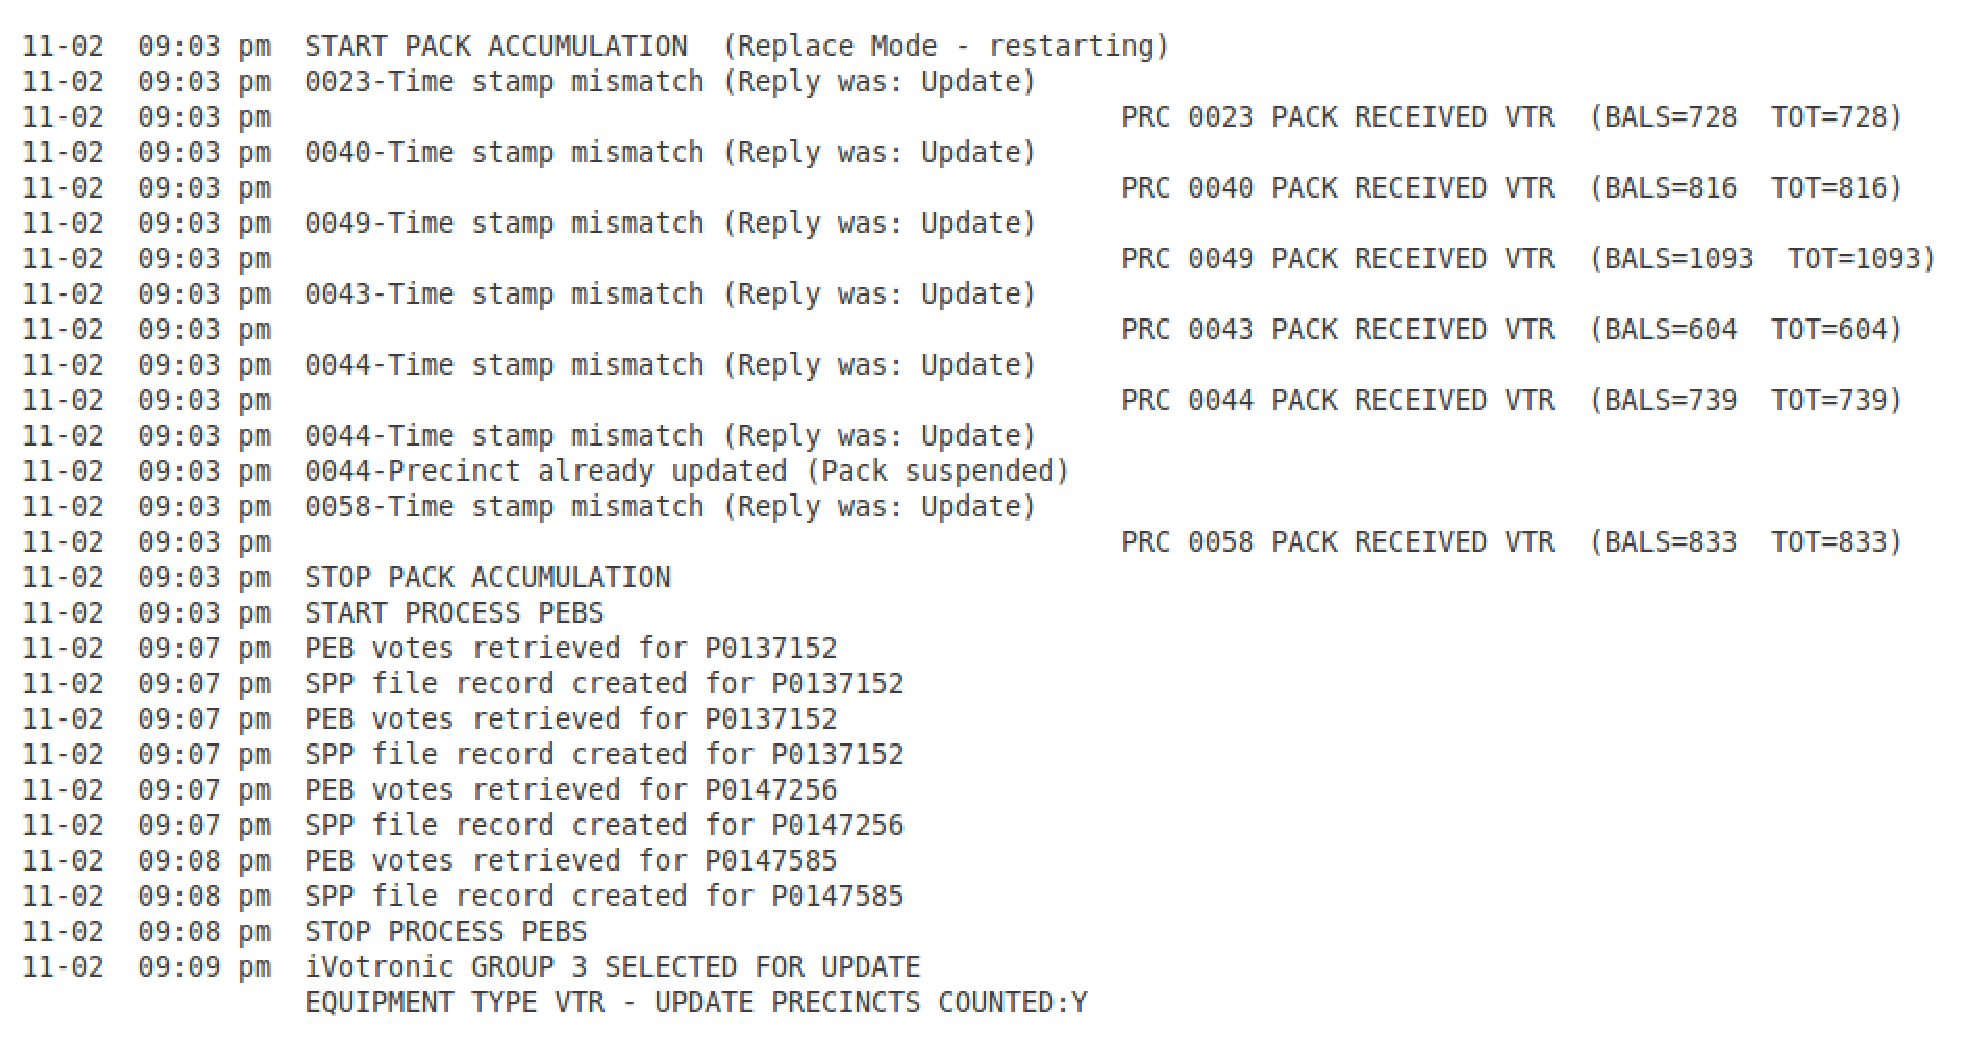
\includegraphics[width=0.7\textwidth]{system}
%This is app~\ref{app:sl}


\end{document}
